%%%%%%%%%%%%%%%%%%%%%%%%%%%%%%%%%%%%%%%%%
% Masters/Doctoral Thesis 
% LaTeX Template
% Version 2.5 (27/8/17)
%
% This template was downloaded from:
% http://www.LaTeXTemplates.com
%
% Version 2.x major modifications by:
% Vel (vel@latextemplates.com)
%
% This template is based on a template by:
% Steve Gunn (http://users.ecs.soton.ac.uk/srg/softwaretools/document/templates/)
% Sunil Patel (http://www.sunilpatel.co.uk/thesis-template/)
%
% Template license:
% CC BY-NC-SA 3.0 (http://creativecommons.org/licenses/by-nc-sa/3.0/)
%
%%%%%%%%%%%%%%%%%%%%%%%%%%%%%%%%%%%%%%%%%

%----------------------------------------------------------------------------------------
%	PACKAGES AND OTHER DOCUMENT CONFIGURATIONS
%----------------------------------------------------------------------------------------

\documentclass[
11pt, % The default document font size, options: 10pt, 11pt, 12pt
openany,
%oneside, % Two side (alternating margins) for binding by default, uncomment to switch to one side
english, % ngerman for German
singlespacing, % Single line spacing, alternatives: onehalfspacing or doublespacing
%draft, % Uncomment to enable draft mode (no pictures, no links, overfull hboxes indicated)
%nolistspacing, % If the document is onehalfspacing or doublespacing, uncomment this to set spacing in lists to single
%liststotoc, % Uncomment to add the list of figures/tables/etc to the table of contents
%toctotoc, % Uncomment to add the main table of contents to the table of contents
%parskip, % Uncomment to add space between paragraphs
%nohyperref, % Uncomment to not load the hyperref package
headsepline, % Uncomment to get a line under the header
%chapterinoneline, % Uncomment to place the chapter title next to the number on one line
%consistentlayout, % Uncomment to change the layout of the declaration, abstract and acknowledgements pages to match the default layout
]{Thesis} % The class file specifying the document structure

\usepackage[utf8]{inputenc} % Required for inputting international characters
\usepackage[T1]{fontenc} % Output font encoding for international characters

\usepackage{mathpazo} % Use the Palatino font by default

\usepackage[backend=bibtex,style=authoryear,natbib=true]{biblatex} % Use the bibtex backend with the authoryear citation style (which resembles APA)

\addbibresource{bibliography.bib} % The filename of the bibliography

\usepackage[autostyle=true]{csquotes} % Required to generate language-dependent quotes in the bibliography

\usepackage{indentfirst}

%----------------------------------------------------------------------------------------
%	MARGIN SETTINGS
%----------------------------------------------------------------------------------------

\geometry{
	paper=a4paper, % Change to letterpaper for US letter
	left=3cm, % Inner margin
	right=3cm, % Outer margin
	% bindingoffset=1cm, % Binding offset
	top=1.5cm, % Top margin
	bottom=1.5cm, % Bottom margin
	%showframe, % Uncomment to show how the type block is set on the page
}

%----------------------------------------------------------------------------------------
%	THESIS INFORMATION
%----------------------------------------------------------------------------------------

\thesistitle{Investigating the Impact of Various Feature Extraction Algorithms on Performance in Automatic Speech Recognition Systems\newline \\
	\large To What Extent Do Mel-Frequency Cepstrum Coefficients Outperform Other Speech Feature Extraction Algorithms in Speech Recognition Neural Networks?}
\supervisor{Courtney \textsc{Edwards}} % Your supervisor's name, this is used in the title page, print it elsewhere with \supname
\degree{International Baccalaureate Programme} % Your degree name, this is used in the title page and abstract, print it elsewhere with \degreename
\author{Daniel \textsc{Lu}} % Your name, this is used in the title page and abstract, print it elsewhere with \authorname

\subject{Computer Sciences} % Your subject area, this is not currently used anywhere in the template, print it elsewhere with \subjectname
\university{\href{https://merivalehs.ocdsb.ca/}{Merivale High School}} % Your university's name and URL, this is used in the title page and abstract, print it elsewhere with \univname

\AtBeginDocument{
\hypersetup{pdftitle=\ttitle} % Set the PDF's title to your title
\hypersetup{pdfauthor=\authorname} % Set the PDF's author to your name
}

\begin{document}

\frontmatter % Use roman page numbering style (i, ii, iii, iv...) for the pre-content pages

\pagestyle{plain} % Default to the plain heading style until the thesis style is called for the body content

%----------------------------------------------------------------------------------------
%	TITLE PAGE
%----------------------------------------------------------------------------------------

\begin{titlepage}
\begin{center}

\vspace*{.06\textheight}
{\scshape\LARGE \univname\par}\vspace{1.5cm} % University name

\HRule \\[0.4cm] % Horizontal line
{\huge \bfseries \ttitle\par}\vspace{0.4cm} % Thesis title
\HRule \\[1.5cm] % Horizontal line
 
\begin{minipage}[t]{0.4\textwidth}
\begin{flushleft} \large
\emph{Author:}\\
{\authorname} % Author name - remove the \href bracket to remove the link
\end{flushleft}
\end{minipage}
\begin{minipage}[t]{0.4\textwidth}
\begin{flushright} \large
\emph{Supervisor:} \\
{\large \supname} % Supervisor name - remove the \href bracket to remove the link  
\end{flushright}
\end{minipage}\\[3cm]
 
\vfill

{\large \today}\\[4cm] % Date

\vfill
\end{center}
\end{titlepage}

%----------------------------------------------------------------------------------------
%	LIST OF CONTENTS/FIGURES/TABLES PAGES
%----------------------------------------------------------------------------------------

\tableofcontents % Prints the main table of contents

%----------------------------------------------------------------------------------------
%	ABBREVIATIONS
%----------------------------------------------------------------------------------------

\begin{abbreviations}{ll} % Include a list of abbreviations (a table of two columns)

\textbf{ASR} & \textbf{A}utomatic \textbf{S}peech \textbf{R}ecognition\\
\textbf{LPC} & \textbf{L}inear  textbf{P}redictive \textbf{C}oding\\
\textbf{DFT} & \textbf{D}iscrete \textbf{F}ourier \textbf{T}ransform\\
\textbf{FFT} & \textbf{F}ast \textbf{F}ourier \textbf{T}ransform\\
\textbf{IFT} & \textbf{I}nverse \textbf{F}ourier \textbf{T}ransform\\
\textbf{HMM} & \textbf{H}idden \textbf{M}arkov \textbf{M}odel\\
\textbf{CTC} & \textbf{C}onnectionist \textbf{T}emporal\textbf{C}lassification\\
\textbf{DDC} & \textbf{D}irected \textbf{D}ialogue \textbf{C}onversations\\
\textbf{NLC} & \textbf{N}atural \textbf{L}anguage \textbf{C}onversations\\
\textbf{NLP} & \textbf{N}atural \textbf{L}anguage \textbf{P}rocessing\\
\textbf{DWT} & \textbf{D}iscrete \textbf{W}avelet \textbf{T}ransform\\
\textbf{PLP} & \textbf{P}erceptual \textbf{L}inear \textbf{P}rediction

\end{abbreviations}

%----------------------------------------------------------------------------------------
%	THESIS CONTENT - CHAPTERS
%----------------------------------------------------------------------------------------

\mainmatter % Begin numeric (1,2,3...) page numbering

\pagestyle{thesis} % Return the page headers back to the "thesis" style

% Include the chapters of the thesis as separate files from the Chapters folder
% Uncomment the lines as you write the chapters

% Chapter Template

\chapter{Introduction} % Main chapter title

\label{Introduction} % Change X to a consecutive number; for referencing this chapter elsewhere, use \ref{ChapterX}

%----------------------------------------------------------------------------------------
%	ABSTRACT
%----------------------------------------------------------------------------------------

\section{Abstract}

Automatic speech recognition (ASR) is the ability of a machine to recognize language from human speech and convert it into written text. Such a task is difficult due to the sheer complexity of any spoken language, as well as the varying and unpredictable nature of different people and their speaking habits. Even big-name companies such as Alphabet, Microsoft, and Baidu, who pride themselves in their sophisticated multi-million dollar speech recognition systems, have been countlessly ridiculed for their misinterpretations. However, due to the endless number of possible and practical applications of ASR technology in our developing world, major corporations still aspire to develop an accurate yet optimized speech recognition system for their products and services. For instance, Baidu spent a total of \$4.7 billion dollars on research and development, of which a large portion headed into developing their voice assistant, DuerOS. Hence, the implementation of ASR can improve the ergonomics of any task that requires human interaction, such as personal assistants, smart healthcare and household appliances, and media transcription to support people with disabilities or language barriers. 
\newline\par
Significant development for ASR began in the 50s, with the innovation of Bell’s Audrey and IBM’s Shoebox. These systems fell into a category of ASR systems that recognized individual words to an isolated vocabulary using manually set parameters for phoneme recognition. By the end of the decade, ASR technology could distinguish words with a maximum of four vowels and nine consonants and by the 80s, systems could recognize up to 3000 words, which is around the vocabulary of a six-year-old child. It wasn’t until the late 90s that researchers transitioned outwards of phoneme detection to Hidden Markov Models (HMM) and focused on natural language processing. Deep learning concepts and technologies emerged and were investigated as a solid alternative to HMMs, to the extent to which it is prominently used today.
\newline\par
However, a plausible deep learning system that can recognize continuous speech within a low margin of error is very strenuous to build. A well-designed system can consist of multiple complex layers that can be very complicated to integrate into one another. Nowadays, large tech companies boast an accuracy of almost 95%, which is still fairly low in the context of deep learning. One of these layers is commonly a feature extraction layer that optimizes an input waveform and isolates the distinct resonant qualities of the human vocal tract. Modern speech recognition models widely use Mel-Frequency Cepstrum Coefficients (MFCC) as a pre-processing layer. Yet, MFCCs often have shortcomings when processing audio signals with excess background noise due to their sensitive nature.

%-----------------------------------
%	RATIONALE
%-----------------------------------
\section{Rationale}

This report aims to investigate the extent to which Mel-Frequency Cepstrum Coefficients outperform other feature extraction methods in automatic speech recognition systems. I will assess the performances of MFCCs, Discrete Wavelet Transforms (DWT), Linear Predictive Coding (LPC), and Perceptual Linear Prediction (PLP), as well as the absence of a feature extraction layer, processed through identical recurrent neural network architectures. From this investigation, I will better understand the effectiveness and limitations of different speech feature extraction methods and inform my forthcoming decisions in ASR neural networks.
% Chapter Template

\chapter{Background} % Main chapter title

\label{Background} % Change X to a consecutive number; for referencing this chapter elsewhere, use \ref{ChapterX}

%----------------------------------------------------------------------------------------
%	ASR
%----------------------------------------------------------------------------------------

\section{Automatic Speech Recognition}

Automatic speech recognition models can be split into two broad categories of complexity. First of all, there is single word classification to an isolated vocabulary where directed dialogue conversations are analyzed; its functionality can be seen in early speech recognition efforts such as IBM’s Shoebox. The other variant is continuous speech recognition, where natural language conversations (NLCs) are processed and transcripted to a vocabulary of around 20,000 to 100,000 words. Many technologies today utilize this system, including video subtitles, voice searching, and customer services at call centres. Directed dialogue classification models can be fairly simple to understand and produce through various feed-forward networks, but natural language networks require the use of recurrent neural networks.

%-----------------------------------
%	RNN
%-----------------------------------
\section{Recurrent Neural Networks}

Recurrent neural networks are a variant of deep learning neural networks that use time-sequential data without a fixed shape. These systems are inspired by the biological composition of neurons in the brain, as humans have learned long ago to adapt their innovations from nature. Each neuron, out of around 100 million, is interconnected to many other neurons and passes a signal via its axon to receiving axon terminals belonging to other neurons. Contrastingly, in an artificial neural network, a combination of weights and biases stacked in layers are constantly optimized through gradient descent to produce a matrix of probabilities that highlight the best possible output the network can generate at its current state (for the case of classification architectures). In each cell, a dot product of the input matrix and the cell’s weight matrix is done and summed with the cell’s bias matrix to create an output matrix of values, fed into all of the nodes in the next layer. At first, these matrices use senseless, randomly generated weights and biases that result in a completely random output. However, as the model calculates its loss from an evaluation of the net deviation of the predicted output from the ground truth, a gradient is formulated that adjusts each layer’s parameters closer to what would create an output with a lower loss. The higher loss an output receives, the greater magnitude of the gradient is passed to backpropagation and the more each node is changed, with the vice versa applying as well.
\par
In a typical multi-layer deep learning neural network, the input and output shape of the model are fixed and have to be set. Since the length of the NLC audio input is indeterminate in this investigation, recurrent neural networks can be used to process continuous speech data that last an indeterminate length of time. RNNs accomplish this task by accepting an input for each time step into a recurrent cell and feeding the cell’s generated output to the succeeding cell through a hidden layer, doing so until the input data is completely used. This results in the coupled nature of a recurrent neural network that enables it to find relationships in continuous data, namely in stock market prediction, and influence future outputs. The framework of a standard RNN cell is laid out below (Figure 1).
\par
The distribution of input data and output data can vary from network to network and is ultimately based on the shape of the input data and the desired shape of the output data. For example, a music generation RNN could take in a dataset of Vivaldi’s works as an input and output an infinite length of completely original Vivaldi-styled music: this model would be classified as a one-to-many RNN structure. The following table (Figure 2) describes four main types of RNN structures that satisfy most machine learning purposes.
\par
Due to the continuous nature of NLC, multiple inputs as the audio data and its respective outputs as phonemes, letters, or words are present. Thus, a many-to-many structure will be used as the framework for this investigation’s experimentation.
\par
However, conventional recurrent neural networks have two major problems that need to be considered: the vanishing and exploding gradient problem, and the long-term dependency on sound signals. The vanishing and exploding gradient problem appear during the backpropagation stage of the network, where a gradient propagates through each cell and updates the weights and biases of each node in order for the network to learn. The problem arises when the number of layers starts to increase and the gradients start to travel and multiplied through more and more layers; when a gradient with a slight deviation from y=x is returned to the first node during backpropagation, it begins to increase or decrease exponentially (dependent on its sign) as it progresses through each cell. Correspondingly, as it reaches near the end of backpropagation, the gradient is either too minuscule to the point where the end weight is scarcely updated at all, or too large where the weight cannot be optimized properly.
\par
Going on, sound signals can take up a significant portion of input data, dependent on sample frequency, as a one-second audio clip of someone dictating a word can take up to 16,000 time steps of data. The extreme short-term memory of a simple hyperbolic tangent recurrent network cannot remember what sound signal was inputted into the cell some 5,000 iterations earlier, to the extent it is significant towards producing the output. This is detrimental towards the ultimate performance of the neural network, as a large segment of a model’s decision on a phoneme, character, or word depends on contextual data beforehand. For example, a model could have a hard time discriminating between the letter “k” and “q” with no context. However, the prerequisite knowledge that it was preceded by a “loo” will likely increase the probability that the following letter is “k”. These two setbacks of recurrent neural networks introduced a revolutionary recurrent cell concept introduced in 1997 and prominently used today, termed the Long Short-Term Memory cell.

%-----------------------------------
%	LSTM
%-----------------------------------
\section{Long Short-Term Memory}

Long Short-Term Memory cells counter the two problems above by incorporating an extra hidden memory state that propagates throughout recurrences of the network. The addition of a memory state that can remember important specifics from many recurrences beforehand and influence the current output. Contrary to the perception-based framework of traditional neural networks, an LSTM cell is much more convoluted and contains substantially more weights and biases in the form of specialized gates (Figure 3). The combination of these properties provides the fundamental framework that conceives the LSTM network’s ability to recognize context-sensitive information and is thus the reason why these networks are the standard for building reliable speech recognition systems. 
\par
A simple speech recognition system is usually composed of two different components; a feature extraction layer and the neural network itself. The purpose of the feature extraction layer is to process the raw input data into a more usable and space-efficient form. In the case of ASR, input data is usually in the form of waveform data embedded in .mp3 or .wav files. This one-dimensional waveform data has several limitations due to having less useful features than a two-dimensional format of audio signals, such as spectrograms. Spectrograms are a visual representation of the amplitudinal spectrum of frequencies of an audio signal with respect to time. These isolated frequency amplitudes are also called the Discrete Fourier Transform (DFT) of an input and they can be extracted via the Fast Fourier Transform (FFT) algorithm, laid out below.
\par
DFTs are frequently used in convolutional neural networks due to their property to be represented as an image and are the reliable standard in terms of extracting audio features from waveform data. In a DFT, the x-axis refers to time and the y-axis refers to the frequency that’s played at a certain point in time, with a lighter colour indicating that the amplitude is larger with regard to magnitude (Figure 4). 

%-----------------------------------
%	Feature Extraction Algorithms
%-----------------------------------
\section{Feature Extraction Algorithms}

However, spectrograms are not very well suited nor optimized for visualizing human speech. For instance, a human voice at a conversational level will normally not exceed a frequency of 500 Hz and fall below 60 Hz and it’s not necessary to include non-phonetically vital properties of speech signals in the input data. Therefore, Mel Frequency Cepstral Coefficients (MFCC) intended to artificially replicate the human hearing system with the assumption that the human ear is a reliable speech recognition system in itself. A precise logarithm function is used to retain the phonetically vital properties of speech signals and plot the result on the Mel scale (Figure 5). 
\par
MFCCs are created first by passing spectrogram data through a precise logarithm function, dubbed the Mel-filter bank, to retain the phonetically vital properties of speech signals while also reducing the number of unwanted frequencies in our input data. The result is plotted to a Mel spectrum and applied to the inverse discrete cosine transform, in which it is finally converted into a cepstrum, the inverse of a spectrum. The result is a set of 10-21 coefficients that ultimately present the main speech features of the original waveform data. MFCC data can also be taken as the derivative of and provide further feature data to feed into the neural network. 
\par
Other speech feature extraction functions that will be investigated are DWT, LPC, and PLP. They are each unique in their own manner but are also very closely related to each other with reference to the algorithms used to create them. Discrete Wavelet Transforms decompose a signal into a set of mutually orthogonal wavelet basis functions. It uses the Short-Time Fourier Transform, a variant of the FFT, which carries out a Fourier transform on a signal split into small windows of fixed duration instead of a specific time instance. Linear Predictive Coding generates coefficients that, similar to MFCCs, reflect the characteristics of a simplified vocal tract model, overall compressing the signal alongside the process. As the name suggests, the method is competent at predicting the future of a random process given past observations. Finally, Perceptual Linear Prediction claims to improve speaker independent recognition performance and outperform LPCs in speech recognition. It first warps the spectrogram along the Bark frequency scale (Figure 6), convolves it with the power spectrum, and performs a cubic-root amplitude compression, ultimately creating the linear prediction model.
% Chapter Template

\chapter{Experiment Materials \& Methodology} % Main chapter title

\label{ExperimentMaterialsMethodology} % Change X to a consecutive number; for referencing this chapter elsewhere, use \ref{ChapterX}

In this paper, heavy importance is placed on primary experimental observations and data. Thus, an LSTM neural network is implemented to perform the investigation, with the use of Google’s Tensorflow machine learning API. Using this API allowed for ease of visualizing performance data and greater freedom in the network’s architecture. The network architecture will remain a control variable throughout all trials. The independent variables are the speech feature extraction algorithms, which include STFT spectrograms, Mel spectrograms, MFCCs, and DWTs. The dependent variables are the loss calculated by connectionist temporal classification (CTC) loss, word error rate (WER), and the time taken by each network when processing the test dataset. WER is calculated by the number of substitutions, insertions, and deletions divided by the number of characters and it is a more accurate metric to assess linguistic proximity than loss~\cite{wang_acero_chelba_2003}.

%----------------------------------------------------------------------------------------
%	ABSTRACT
%----------------------------------------------------------------------------------------

\section{Datasets Used}

The LJ Speech Dataset is used to train the neural network that conducted the experiment~\cite{ito_johnson_2017}. The dataset contains 13,100 NLC audio clips of around 4-8 seconds that are spoken by a single speaker reading from a selection of non-fiction literature~\cite{ito_johnson_2017}, amounting to a total of approximately 24 hours of data. 10\% of this data is used for validation while 90\% is fed into training. All in all, there is an average of ~17 words that are spoken in each ~6-second clip and there are around 13,800 distinct words said among all the audio clips~\cite{ito_johnson_2017}.

%-----------------------------------
%	PRE-PROCESSING
%-----------------------------------
\section{Pre-Processing}

The dataset provided the sound files in wav format, which made it very simple to extract its waveform data. Tensorflow’s audio analysis library in combination with PyWavelets~\cite{lee_gommers_waselewski_wohlfahrt_oleary_2019} performs each speech feature extraction algorithm on every sample in the dataset to obtain the respective input data (Figure~\ref{fig:MelSample}).

\begin{figure}[th]
    \centering
    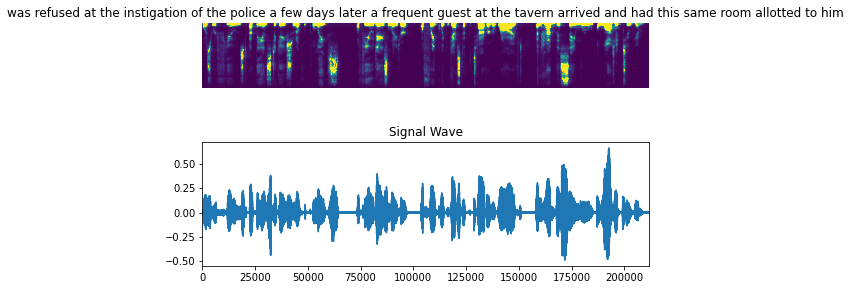
\includegraphics[width=0.9\textwidth]{Figures/melsample.png}
    \decoRule
    \caption[Mel Sample]{Sample of training data paired with its transcription, visualized as a Mel Spectrogram using Tensorflow’s signal library and its respective signal wave}
    \label{fig:MelSample}
\end{figure}

%-----------------------------------
%   NETWORK ARCHITECTURE
%-----------------------------------
\section{Network Architecture}

This report uses an end-to-end recurrent character-based neural network that consists of two convolutional layers, five layers of bidirectional LSTM cells, a dense layer, and a decoding layer to process and display the final output. The LSTM layers take in a time step of data (whose shape is dependent on the feature extraction algorithm), utilize 128 hidden units in each cell and output a one-hot matrix of shape (31, 1) at each time step. The output is a probability matrix of 31 characters that the model predicts the audio signal refers to at that point in time, which includes all of the Latin alphabet, three punctuation marks, as well as a space and a blank character. A character classification system is used over phoneme-based or word-based systems since with the current LSTM network architecture, it is capable of distinguishing between similar-sounding characters in the English dataset used. A working result of this model would output a sequence of slurred letters that, once decoded with CTC loss, would output a word; the model could output “b\_uu\_t\_  \_n\_oo”, which suggests that the original audio input is of a person uttering “but no”~\cite{graves_fernández_gomez_schmidhuber_2006,scheidl_2018}. After this procedure, these characters can be fed into an English language model to be further refined into comprehensible written text as the final output. Refer to~\autoref{AppendixC} for model details.
\par
The LSTM model is trained on 389 batches of training data with each batch consisting of 32 audio clips. The model is trained for 5 epochs for each set of independent variables, with a learning rate of 0.0001 to avoid overfitting, and evaluated by three validation datasets. Each of the three trials holds 21 batches of data that determine the accuracy of each model.
\par
Regarding the feature extraction algorithms, the MFCC trials will have 21 coefficients and the DWT trials will use a biorthogonal 6.8 wavelet (Figure~\ref{fig:MelSample}).

\begin{figure}[th]
    \centering
    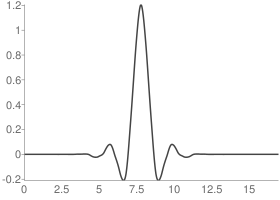
\includegraphics[width=0.5\textwidth]{Figures/wavelet.png}
    \decoRule
    \caption[Bior Wavelet]{A biorthogonal 6.8 wavelet, visualized (Source: Waselewski~\cite{wasilewski_2008})}
    \label{fig:BiorWavelet}
\end{figure}

%-----------------------------------
%	EXPERIMENTAL PROCESS
%-----------------------------------
\section{Experimental Process}

It is essential to clarify some notable semantics of this investigation. The general performance of a model within this investigation is assessed on a synthesis of its accuracy and its efficiency as well as how it compares with other models, though with the greatest emphasis on accuracy. The accuracy of a model is calculated appertaining to both its loss from CTC and its word error rate, and the efficiency of a model is gauged on a comparison of its estimated time complexity and a measured difference of time. For each speech feature extraction algorithm, there will be three trials held, amounting to a total of 4 models and 12 trials.  
% Chapter Template

\chapter{Experimental Results} % Main chapter title

\label{Results} % Change X to a consecutive number; for referencing this chapter elsewhere, use \ref{ChapterX}

%----------------------------------------------------------------------------------------
%	TABULAR PRESENTATION OF DATA
%----------------------------------------------------------------------------------------

\section{Tabular Presentation of Data}

The tables in \autoref{AppendixA} and \autoref{AppendixB} show the raw experimental results of all the trials, with each table presenting the performance of each feature extraction algorithm in pre-processing speech for ASR neural networks.

%-----------------------------------
%	GRAPHICAL PRESENTATION OF DATA
%-----------------------------------

\section{Graphical Presentation of Data}

\begin{figure}[th]
    \centering
    \includesvg[width=\textwidth]{Figures/SpectrogramEpochLoss.svg}
    \caption[Spectrogram]{Spectrogram}
    \label{fig:SpectrogramEpochLoss}
\end{figure}

\begin{figure}[th]
    \centering
    \includesvg[width=\textwidth]{Figures/MelSpectrogramEpochLoss.svg}
    \caption[Mel Spectrogram]{Mel Spectrogram}
    \label{fig:MelSpectrogramEpochLoss}
\end{figure}

\begin{figure}[th]
    \centering
    \includesvg[width=\textwidth]{Figures/MFCCEpochLoss.svg}
    \caption[MFCC]{MFCC}
    \label{fig:MFCCEpochLoss}
\end{figure}

\begin{figure}[th]
    \centering
    \includesvg[width=\textwidth]{Figures/DWTEpochLoss.svg}
    \caption[DWT]{DWT}
    \label{fig:DWTEpochLoss}
\end{figure}

\begin{figure}[th]
    \centering
    \includesvg[width=\textwidth]{Figures/ComparisonOfTime.svg}
    \caption[Execution Times]{Execution Times}
    \label{fig:ExecutionTimes}
\end{figure}
% Chapter Template

\chapter{Analysis \& Conclusions} % Main chapter title

\label{AnalysisConclusions} % Change X to a consecutive number; for referencing this chapter elsewhere, use \ref{ChapterX}

%----------------------------------------------------------------------------------------
%	EXPERIMENTAL ANALYSIS AND TRENDS
%----------------------------------------------------------------------------------------

\section{Experimental Analysis and Trends}

\begin{figure}[th]
    \centering
    \includesvg[width=\textwidth]{Figures/ComparisonOfAccuracy.svg}
    \caption[ComparisonOfAccuracy]{A comparison of extraction algorithms’ accuracies against each other}
    \label{fig:ComparisonOfAccuracy}
\end{figure}

In the visualizations of the experiment results above, much can be inferred about how differing feature extraction algorithms perform against each other. As observed in (Figure~\ref{fig:ComparisonOfAccuracy}), spectrograms, Mel spectrograms, and MFCCs performed similarly, with similar results in loss and WER, while DWT’s performance is noticeably worse than any other algorithm in terms of both accuracy and time spent. While other speech extraction algorithms had an ending WER of roughly 63\%, DWT’s average WER in epoch 5 is 74\%. DWT’s poor performance could be attributed to two possible causes: either the algorithm is inefficient in extracting audio features or there is error present in implementing the algorithm. DWT outputs coefficients whose values indicate the overall resemblance of a wavelet to any window of a specific waveform. The number of coefficients can vary but are generally very low compared to the number of data present in spectrograms, resulting in an inevitably lossy output within this investigation. Additionally, it is the sole algorithm that did not use Tensorflow’s signal library and instead PyWavelets, which may have caused the significant disparity in execution time; this factor is further elaborated below.
\par
Concerning the performances of spectrograms, Mel spectrograms, and MFCCs, it is seen in (Figure~\ref{fig:ComparisonOfAccuracy}) and (Figure~\ref{fig:ExecutionTimes}) that their accuracies and times are very similar, but have small discrepancies that are important to distinguish. Mel spectrograms and MFCCs generally achieve better validation loss than raw spectrograms by a value of ~4 while spectrograms and Mel spectrograms have slightly lower word error rates than MFCCs, by nearly 2\%. Since the performance of Mel spectrograms remained consistently efficient in both metrics of accuracy, Mel spectrograms overall performed the best among all feature extraction algorithms explored in this study, though to a little extent.
\par
Furthermore, comparing the time complexity of each algorithm reveals that MFCCs are the most efficient. This could be a result of the less trainable parameters needed in the neural network to process the compressed output of MFCCs. To elaborate, a time step of data produced with MFCC that is passed to an LSTM cell would consume around 21n spaces of data, with n being the number of time steps. In contrast, a spectrogram would normally take up nearly 193n spaces of data per time step\footnote{For a frame step of 160, frame length of 256, and fast Fourier transform length of 384}, depending on the frequency range desired while computing the STFT, which would require levels of magnitude higher levels of computing required to process an audio signal.

%-----------------------------------
%	FURTHER RESEARCH OPPORTUNITIES AND ASPIRATIONS
%-----------------------------------

\section{Further Research Opportunities and Aspirations}

The experimental process could be improved, as it led to a few sources of error: the first of which lies in the consistency of the speed of the computer the tests were run on. In Table~\ref{spectro_time} and~\ref{dwt_time} found in \autoref{AppendixB}, the large standard deviation of the spectrogram and DWT trials shows that there is a large uncertainty in measuring execution time can exist, possibly due to the varied use of the training CPU that occurred during the trials. This error can be disregarded if an uncertainty of ±1 second is added to the running times of each trial as a result of systematic irregularity in hardware.
\par
Another source of error mentioned above is the inconsistency in the selection of audio processing libraries used to carry out the feature extraction algorithms. Consequently from the limited number of options available on any single audio analysis library that doesn’t include the entirety of my independent variables, such as Librosa, multiple libraries had to be used, which altogether reduces the uniformity within my methodology. This error can be eliminated by implementing the algorithms manually without using third-party libraries.
\par
To expand the scope of future investigations regarding the research topic, there are several improvements that could be implemented. To attain more accurate, representative data and better overall performance of each algorithm in the neural network, more epochs of training data could have been trained if hardware limitations were not present. Additionally, a downside of the current dataset is that all of the NLC speech is spoken by one speaker, which is unrealistic in practical scenarios. Obtaining a dataset with a variety of speakers would better reflect the performances of these algorithms through more realistic analyses.\\
\par
There are several research opportunities that could be explored regarding the research question. The speech feature extraction algorithms examined in this paper are a portion of the most conventionally used computer scientists use today for speech recognition. Even so, there are some modern and advanced yet ambiguous speech feature extraction algorithms out there that may perform even better than the ones investigated in this report but don’t have the recognition to gain traction in the field of ASR. Investigating the extent to which these are viable as a replacement for MFCCs could yield interesting results. 
\par
In the future, it would be worthwhile to examine the extent to which MFCCs can perform well in noise-heavy environments with the addition of white noise and the use of noise reduction/cancellation systems; the experimental results currently presented do not draw out clear conclusions on whether MFCCs should be used if a system expects a high magnitude of background noise.

%-----------------------------------
%	CONCLUSIONS
%-----------------------------------

\section{Conclusions}

This paper presented several conclusions regarding the research question at hand through an analysis of the performances of different speech feature extraction algorithms. The results show that although MFCCs are considerably optimized and contain denser key vocal information of a waveform, Mel spectrograms overall possess the highest degree of accuracy while maintaining a reasonable processing time with large inputs. In a more practical sense, the use of spectrograms, Mel spectrograms, and MFCCs are generally all viable within a speech feature extraction layer in most non-industry ASR neural networks. 
\include{Sections/WorksCited} 

%----------------------------------------------------------------------------------------
%	THESIS CONTENT - APPENDICES
%----------------------------------------------------------------------------------------

\appendix % Cue to tell LaTeX that the following "chapters" are Appendices

% Include the appendices of the thesis as separate files from the Appendices folder
% Uncomment the lines as you write the Appendices

% Appendix A

\chapter{Frequently Asked Questions} % Main appendix title

\label{AppendixA} % For referencing this appendix elsewhere, use \ref{AppendixA}

\section{How do I change the colors of links?}

The color of links can be changed to your liking using:

{\small\verb!\hypersetup{urlcolor=red}!}, or

{\small\verb!\hypersetup{citecolor=green}!}, or

{\small\verb!\hypersetup{allcolor=blue}!}.

\noindent If you want to completely hide the links, you can use:

{\small\verb!\hypersetup{allcolors=.}!}, or even better: 

{\small\verb!\hypersetup{hidelinks}!}.

\noindent If you want to have obvious links in the PDF but not the printed text, use:

{\small\verb!\hypersetup{colorlinks=false}!}.

%% Appendix A

\chapter{Appendix B - Execution Time} % Main appendix title

\label{AppendixB} % For referencing this appendix elsewhere, use \ref{AppendixA}

\begin{table}[!ht]
    \centering
    \caption{Spectrogram Execution Time}
    \begin{adjustbox}{width=\textwidth,keepaspectratio}
    \begin{tabular}{|l|l|l|l|l|l|l|}
    \hline
        \textbf{Epoch} & \textbf{1} & \textbf{2} & \textbf{3} & \textbf{4} & \textbf{5} & \textbf{Average} \\ \hline
        \textbf{Trial 1} & 52.4 & 51.5 & 51.4 & 51.5 & 51.5 & ~ \\ \hline
        \textbf{Trial 2} & 53 & 48.9 & 55.8 & 55.3 & 55.3 & ~ \\ \hline
        \textbf{Trial 3} & 46.5 & 44.2 & 43.1 & 40.6 & 45.2 & ~ \\ \hline
        \textbf{Average Execution Time (s)} & 50.63333333 & 48.2 & 50.1 & 49.13333333 & 50.66666667 & 49.74666667 \\ \hline
    \end{tabular}
    \end{adjustbox}
    \label{spectro_time}
\end{table}

\begin{table}[!ht]
    \centering
    \caption{Mel Spectrogram Execution Time}
    \begin{adjustbox}{width=\textwidth,keepaspectratio}
    \begin{tabular}{|l|l|l|l|l|l|l|}
    \hline
        \textbf{Epoch} & \textbf{1} & \textbf{2} & \textbf{3} & \textbf{4} & \textbf{5} & \textbf{Average} \\ \hline
        \textbf{Trial 1} & 52.7 & 52.3 & 51.8 & 51.8 & 53.8 & ~ \\ \hline
        \textbf{Trial 2} & 55.1 & 53.2 & 54.2 & 51.8 & 52.9 & ~ \\ \hline
        \textbf{Trial 3} & 52.8 & 51 & 50.2 & 50 & 50.7 & ~ \\ \hline
        \textbf{Average Execution Time (s)} & 53.53333333 & 52.16666667 & 52.06666667 & 51.2 & 52.46666667 & 52.28666667 \\ \hline
    \end{tabular}
    \end{adjustbox}
    \label{melspectro_time}
\end{table}

\begin{table}[!ht]
    \centering
    \caption{MFCC Execution Time}
    \begin{adjustbox}{width=\textwidth,keepaspectratio}
    \begin{tabular}{|l|l|l|l|l|l|l|}
    \hline
        \textbf{Epoch} & \textbf{1} & \textbf{2} & \textbf{3} & \textbf{4} & \textbf{5} & \textbf{Average} \\ \hline
        \textbf{Trial 1} & 49.5 & 48.6 & 48.6 & 48 & 48.2 & ~ \\ \hline
        \textbf{Trial 2} & 48.4 & 46.7 & 46.9 & 46.9 & 47 & ~ \\ \hline
        \textbf{Trial 3} & 50.3 & 47.1 & 47.1 & 46.9 & 47.1 & ~ \\ \hline
        \textbf{Average Execution Time (s)} & 49.4 & 47.46666667 & 47.53333333 & 47.26666667 & 47.43333333 & 47.82 \\ \hline
    \end{tabular}
    \end{adjustbox}
    \label{mfcc_time}
\end{table}

\begin{table}[!ht]
    \centering
    \caption{DWT Execution Time}
    \begin{adjustbox}{width=\textwidth,keepaspectratio}
    \begin{tabular}{|l|l|l|l|l|l|l|}
    \hline
        \textbf{Epoch} & \textbf{1} & \textbf{2} & \textbf{3} & \textbf{4} & \textbf{5} & \textbf{Average} \\ \hline
        \textbf{Trial 1} & 85.2 & 83.4 & 77.6 & 69 & 57.2 & ~ \\ \hline
        \textbf{Trial 2} & 78.5 & 64.9 & 66.1 & 71.8 & 73.9 & ~ \\ \hline
        \textbf{Trial 3} & 88.5 & 52.7 & 53.3 & 53.5 & 83.5 & ~ \\ \hline
        \textbf{Average Execution Time (s)} & 84.06666667 & 67 & 65.66666667 & 64.76666667 & 71.53333333 & 70.60666667 \\ \hline
    \end{tabular}
    \end{adjustbox}
    \label{dwt_time}
\end{table}
%% Appendix A

\chapter{Appendix C - Model Graph} % Main appendix title

\label{AppendixC} % For referencing this appendix elsewhere, use \ref{AppendixA}

\begin{table}[!ht]
    \centering
    \caption{Sample Network Architecture for Spectrogram}
    \begin{tabular}{|l|l|l|}
    \hline
        \textbf{Layer (Type)} & \textbf{Output Shape} & \textbf{Number of Parameters} \\ \hline
        input (InputLayer) & "(None, None, 193)" & 0 \\ \hline
        expand\_dim (Reshape) & "(None, None, 193, 1)" & 0 \\ \hline
        conv\_1 (Conv2D) & "(None, None, 97, 32)" & 14432 \\ \hline
        conv\_1\_bn (BatchNormalization) & "(None, None, 97, 32)" & 128 \\ \hline
        conv\_1\_relu (ReLU) & "(None, None, 97, 32)" & 0 \\ \hline
        conv\_2 (Conv2D) & "(None, None, 49, 32)  " & 236544 \\ \hline
        conv\_2\_bn (BatchNormalization) & "(None, None, 49, 32)  " & 128 \\ \hline
        conv\_2\_relu (ReLU) & "(None, None, 49, 32)  " & 0 \\ \hline
        reshape\_1 (Reshape) & "(None, None, 1568)" & 0 \\ \hline
        bidirectionalLSTM\_1 (Bidirectional) & "(None, None, 1024)" & 8523776 \\ \hline
        dropout (Dropout) & "(None, None, 1024)" & 0 \\ \hline
        bidirectionalLSTM\_2 (Bidirectional) & "(None, None, 1024)" & 6295552 \\ \hline
        dropout\_1 (Dropout) & "(None, None, 1024)" & 0 \\ \hline
        bidirectionalLSTM\_3 (Bidirectional) & "(None, None, 1024)" & 6295552 \\ \hline
        dropout\_2 (Dropout) & "(None, None, 1024)" & 0 \\ \hline
        bidirectionalLSTM\_4 (Bidirectional) & "(None, None, 1024)" & 6295552 \\ \hline
        dropout\_3 (Dropout) & "(None, None, 1024)" & 0 \\ \hline
        bidirectionalLSTM\_5 (Bidirectional) & "(None, None, 1024)" & 6295552 \\ \hline
        dense\_1 (Dense) & "(None, None, 1024)" & 1049600 \\ \hline
        dense\_1\_relu (ReLU) & "(None, None, 1024)" & 0 \\ \hline
        dropout\_4 (Dropout) & "(None, None, 1024)" & 0 \\ \hline
        dense (Dense) & "(None, None, 32) " & 32800 \\ \hline
        \textbf{Total parameters} & ~ & 35039616 \\ \hline
    \end{tabular}
    \label{model}
\end{table}

\begin{figure}[th]
    \centering
    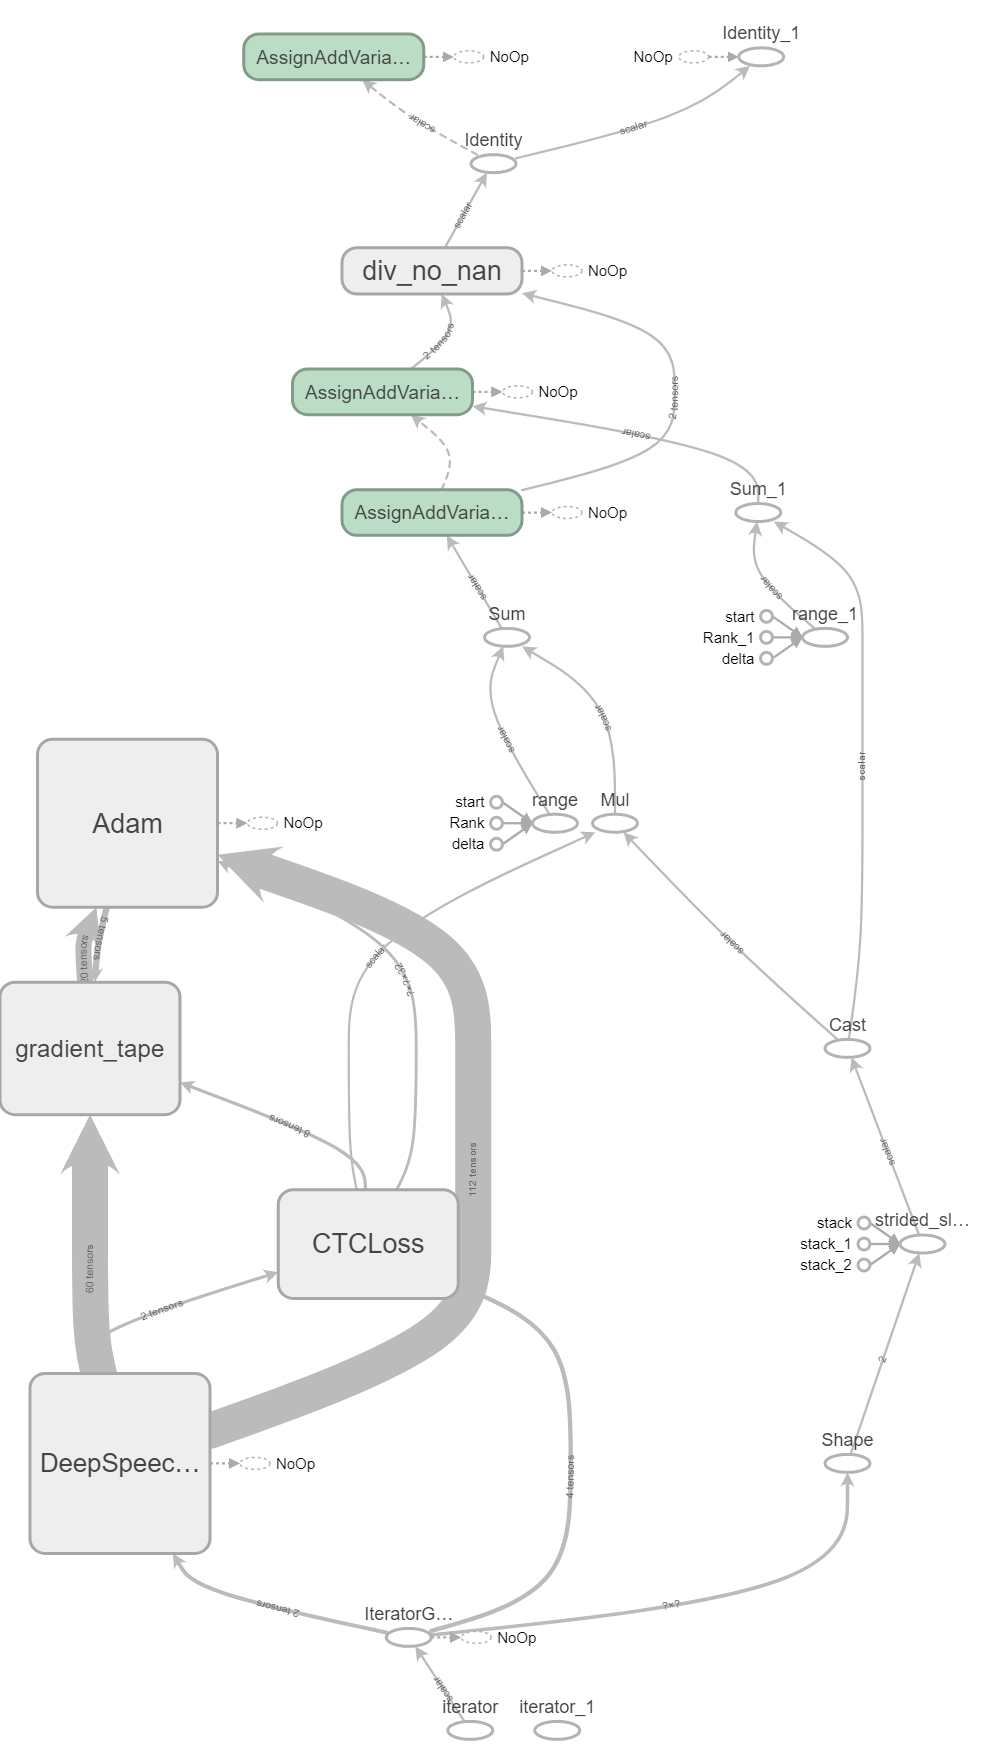
\includegraphics[width=0.7\textwidth]{Figures/model.png}
    \caption[TensorflowModelGraph]{A graph of the general Tensorflow model used in this investigation - deep speech is the name of the neural network outlined above}
    \label{fig:TensorflowModelGraph}
\end{figure}


%----------------------------------------------------------------------------------------
%	BIBLIOGRAPHY
%----------------------------------------------------------------------------------------

\printbibliography

%----------------------------------------------------------------------------------------

\end{document}